\section{Empirical specification}
\label{app:empirical}
\subsection{Observations}
For a contract opening at $o$ and closing at $o+900$ seconds, the candle ending at $o+60k$ gives the transaction close $p_{k-1}$ and the traded quantity $v_{k-1}$, $k\geq1$. A forecast issued $\ell$ minutes before close uses candles ending at or before $o+900-60(\ell+1)$, giving prices $p_0,\ldots,p_T$ with $T=8$ for $\ell=5$ and $T=12$ for $\ell=1$. Increments are $z_t=\logit\bar p_t-\logit\bar p_{t-1}$ with $\bar p=\min\{\max\{p,\epsilon\},1-\epsilon\}$, and $z_t$ is paired with the volume $v_t$ of the candle that closes it. The primary clipping is $\epsilon=0.001$ and the sensitivity is $\epsilon=0.005$. Every model and comparator is fitted separately for each lead and clipping level, and by asset where stated.

\subsection{Mixture}
Pool the training increments and set $s=\max\{1.4826\operatorname{MAD}(z),0.05\}$. Let $m_v$ be the median positive training volume, $r=v/m_v$ and $g(r)=2r/(1+r)$. The catalogue is the Cartesian product $w\in\{0.2,0.5,0.8\}$, $a\in\{0,0.1,0.3,0.6\}$, twelve states shared by all increments of a path. With $q=2y-1$ and $\mu_j=a_js$, the gates are the normalized values of
\[
 \bigl(w_j(1+r)^{1/2},\ (1-w_j)(1+r)^{3/10}/2,\ (1-w_j)/2\bigr)
\]
and the components are
\[
 N\!\Bigl(q\mu_jg(r),\frac{s^2}{1+0.25r}\Bigr),\qquad N\!\bigl(-0.5q\mu_jg(r),s^2\bigr),\qquad t_5\bigl(0,s\sqrt{3/5}\bigr),
\]
with variances in the Gaussian arguments. The no-volume variant sets $r\equiv1$ in fitting and prediction. The catalogue masses $\pi$ maximize the training conditional likelihood $\sum_i\log\sum_j\pi_j\prod_tf_{y_i,j}(z_{it}\mid v_{it})$ plus $(1/12)\sum_j\log\pi_j$ by EM from $\pi_j=1/12$, stopping when the relative objective change is below $10^{-9}$ or after 2,000 iterations. The forecast is $\operatorname{expit}\{\logit p_Y+B_M\}$, where $B_M=\log\{\sum_j\pi_j\prod_tf_{1,j}\}-\log\{\sum_j\pi_j\prod_tf_{0,j}\}$ is the log Bayes factor, with $p_Y=(\sum_iy_i+0.5)/(n+1)$. All fits converged (388 and 191 iterations at the two leads with volume, 500 and 250 without). Fitted values at $\epsilon=0.001$ are $s=0.490$ and $0.603$ and $m_v=19{,}677$ and $24{,}088$ contracts. At the five-minute lead the masses concentrate on $(w,a)=(0.2,0)$, $(0.2,0.6)$ and $(0.5,0.6)$, with $0.28$, $0.23$ and $0.44$.

\subsection{Comparators}
Logistic models standardize features $u_i$ with the means and standard deviations of their fitting sample and minimize the summed objective
\[
 \sum_{i=1}^n\bigl[\log\{1+e^{\beta_0+\beta^{\mathsf T}u_i}\}-y_i(\beta_0+\beta^{\mathsf T}u_i)\bigr]+\frac\lambda2\|\beta\|_2^2
\]
by L-BFGS, with the intercept $\beta_0$ unpenalized. $P_{\rm lin}$, $H_{\rm log}$ and $E_{\rm log}$ are fitted on training data with the penalty from $\{0.01,0.1,1,10\}$ minimizing validation log loss. $P_{\rm cub}$ and the combinations are fitted on validation data with $\lambda=1$. The features of $P_{\rm cub}$ are $x_T,x_T^2,x_T^3$, the asset indicator, and its products with the three powers, so it has an asset-specific intercept and cubic. In the combinations, $B_M$ or $B_G$ is one further feature. In $H_{\rm log}$ the volume features use $\log(1+v_t)$ over all retained candles, the slope is its least-squares slope on centered time, and the volume-weighted increment is $\sum_tz_tv_t/\sum_tv_t$. The Gaussian history model fits, per asset, class means $m_0,m_1$ and the shared covariance $0.9S+0.1\operatorname{diag}(S)$ of within-class residuals, with diagonal floor $10^{-4}$, and uses $B_G=(z-(m_0+m_1)/2)^{\mathsf T}\Sigma^{-1}(m_1-m_0)$ with an asset-specific smoothed prior.

\subsection{Original-window scores}
\begin{table}[h]
\caption{Held-out losses on the same 664 contracts at each lead (14 UTC dates, 332 contracts per asset). Lower is better. Names follow Table~\ref{tab:infosets}.}
\label{tab:empirical-scores}
\centering\scriptsize
\begin{tabular}{lrrrr}
\toprule
 & \multicolumn{2}{c}{5-minute lead} & \multicolumn{2}{c}{1-minute lead} \\
Method & Brier & Log loss & Brier & Log loss \\
\midrule
Training frequency & 0.2506 & 0.6944 & 0.2506 & 0.6944 \\
Initial price & 0.2303 & 0.6520 & 0.2303 & 0.6520 \\
$P_{\rm last}$, latest price & 0.1271 & 0.3998 & 0.0655 & 0.2138 \\
$P_{\rm lin}$, linear price calibration & 0.1255 & 0.3941 & 0.0649 & 0.2120 \\
$P_{\rm cub}$, cubic price calibration & 0.1290 & 0.4042 & 0.0655 & 0.2117 \\
$H_{\rm log}$, history logistic & 0.1263 & 0.3968 & 0.0694 & 0.2232 \\
$M$, mixture & 0.1923 & 0.5660 & 0.1495 & 0.4695 \\
$M_0$, mixture without volume & 0.1442 & 0.4431 & 0.0855 & 0.2835 \\
$P_{\rm cub}{+}M$ & 0.1289 & 0.4041 & 0.0656 & 0.2119 \\
$P_{\rm cub}{+}M_0$ & 0.1299 & 0.4060 & 0.0655 & 0.2120 \\
$G$, joint Gaussian history & 0.1355 & 0.4168 & 0.0766 & 0.2500 \\
$P_{\rm cub}{+}G$ & 0.1310 & 0.4083 & 0.0676 & 0.2174 \\
$E_{\rm log}^\dagger$, matched endpoint logistic & 0.1258 & 0.3955 & 0.0657 & 0.2139 \\
\bottomrule
\end{tabular}

\end{table}

\subsection{Sensitivity and diagnostics}
At the five-minute lead no observed price lies outside $[0.005,0.995]$, so both clipping levels give identical results. At the one-minute lead, with $\epsilon=0.005$, the scores of Table~\ref{tab:empirical-scores} change by less than $0.001$ in Brier loss. The mixture minus $P_{\rm lin}$ is $+0.0848$ ($[+0.0697,+0.1002]$) and $P_{\rm cub}{+}M$ minus $P_{\rm cub}$ is $+0.00016$ ($[-0.00016,+0.00043]$). Table~\ref{tab:validation-bins} gives the validation diagnostic by initial price.

\begin{table}[h]
\caption{Validation window, five-minute lead: mean forecast and Brier loss of the mixture $M$ and of $P_{\rm lin}$ by initial-price bin.}
\label{tab:validation-bins}
\centering\scriptsize
\begin{tabular}{lrrrrrr}
\toprule
$p_0$ bin & $n$ & Outcome rate & Mean $M$ & Mean $P_{\rm lin}$ & Brier $M$ & Brier $P_{\rm lin}$ \\
\midrule
$<0.30$ & 14 & 0.357 & 0.457 & 0.288 & 0.220 & 0.133 \\
$[0.30,0.45)$ & 162 & 0.333 & 0.451 & 0.364 & 0.215 & 0.129 \\
$[0.45,0.55)$ & 258 & 0.484 & 0.486 & 0.504 & 0.196 & 0.133 \\
$[0.55,0.70)$ & 209 & 0.569 & 0.522 & 0.632 & 0.192 & 0.137 \\
$\geq0.70$ & 21 & 0.714 & 0.531 & 0.747 & 0.162 & 0.064 \\
\bottomrule
\end{tabular}

\end{table}

\begin{figure}[h]
\centering
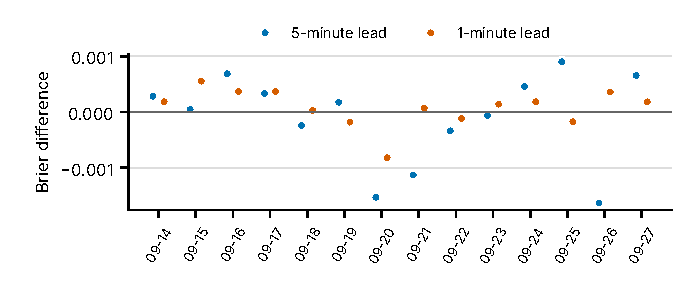
\includegraphics[width=0.72\linewidth]{generated/date_differences.pdf}
\caption{Date-level mean Brier difference, $P_{\rm cub}{+}M$ minus $P_{\rm cub}$, on the 14 test dates.}
\label{fig:dates}
\end{figure}

\subsection{Artifact}
The anonymized artifact contains the collection scripts with checksummed raw responses, the protocol and model-design documents written before collection, the evaluation and model code with tests, the frozen fitted models and prediction lock, the held-out predictions and scores, and the scripts for every figure and diagnostic in this paper.
